\setstretch{1.6}
\sectiontitle{6}{Tip Tracking Integration}
\lhead{Tip Tracking Integration} % section header

\subsection{Theory}


\subsection{Methods}

\subsubsection{Refactoring of Vision Code}
As mentioned in the project context there was an existing 3D tip tracking algorithm that was developed in python specifically for this project. However it was all implemented in a single file and had not been tested for real-time scenarios, and since the code used YOLO (\todo{explanation of yolo})for object detection it was necessary to not only restructure the code for real-time use, but also to thread it to minimize latencies that would otherwise have rendered the code unusable for real-time feedback, communication between this python code and the controlsystem in Qt also had to be implemented, therefore it was decided that a full restructuring of the code was necessary
\todo{insert figure of old vision structure}. The code was refactored using the some code quality criteria as discussed in the theory section on refactoring. 
\newline \newline
As the project progressed it became clear that the 3D vision system using 

\subsubsection{Choosing a Communication Protocol}
In order to establish a robust connection between the already existing Python-based tip tracking system and the C++/Qt-based control system several ways of establishing an interface were evaluated. In order to choose the most suited communication method a set of evaluation criteria based on their suitability for real-time dat streaming \textit{Designing Data Intensive Applications} \cite{kleppmann_designing_2017} were used.

\begin{enumerate}
    \item \textbf{Latency and Real-Time Performance} - The ability to provide low-latency communication suitable for real-time control.
    \item \textbf{Fault Tolerance and Robustness} - Resiliance to failures such as dropped messages or system crashes.
    \item \textbf{Communication Model} - Suitability for push-based (streaming) or pull.based (request-response) communication
    \item \textbf{Message Format and Serialization} - Efficiency of data encoding and compatibility across languages.
    \item \textbf{Ordering and Consitency Guarantees} - The ability to ensure data arrives in the correct order.
    \item \textbf{Scalability} - The capability to accommodate future system expansions, such as integrating communication with a potential real-time path planning algorithm.
    \item \textbf{Ease of Implementation and Maintenance} - Complexity of integrating the communication method into the existing system.
\end{enumerate}

There are several ways to establish a communication layer that allows real-time data transfer between two programs. This includes ...


\subsubsection{Tip tracking interface evaluation}
Several methods exist for enabling real-time inter-process communication or networking-based communication. The choice of method impacts the systems performance, reliability and scalability. The primary methods considered for data exchange between the vision system and the control system are

\paragraph*{File-based communication}
The simplest solution in terms of implementation is file based communication. The vision system would for each detection write to a file which is subsequently read by the control system. This requires the control system to continuously monitor the file for updates introducing latency that is further exacerbated by file system access times and disk I/O overhead. 

In terms of fault tolerance, file-based communication has the benefit of data persisting even if a process crashes, however it is not designed for high-frequency updates. Race conditions can occur if both the vision and control systems attempt to access the file simultaneously. Locking mechanisms can mitigate this, but at the cost of further increasing latency. This method was therefore concluded to not be a viable solution due to its high latency and inefficient real-time performance.

\paragraph*{Shared memory}
A significantly faster method is shared memory. Shared memory allows multiple processes to access a common memory space, enables rapid data exchange without the overhead of disk I/O or network communication. However it also introduces concurrency and data consistency challenges. 

Since multiple processes may attempt to read and write simultaneously, synchronization mechanisms such as mutexes or semaphores are required to prevent race conditions. This adds complexity and thus makes the system less robust and maintainable. Another challenge is that shared memory must be allocated and managed by both processes. This makes it difficult to integrate across different programming languages where data structures may not be inherently compatible. Thus the complexity, lack of language compatibility and make it impractical for this application.

\paragraph*{Named Pipes}
Named Pipes allow data to be transmitted between processes on the same machine asynchronously by operating as a first-in, first-out (FIFO) buffer. Compared to file-based communication, pipes offer lower latency and are more efficient for continuous data streaming. The main limitation in the context of this project is that they are constrained to a single machine. This limits the scalability since in a later revision one might want to run the vision and control systems on separate machines in a distributed setup. 

\paragraph*{Message queues}
Message queues provide structured message passing using a queue-based architecture \todo{cite}. Systems such as RabbitMQ and Apache Kafka provide reliable message delivery making message queues highly fault tolerant. However they also introduce latency due to message buffering and broker management \todo{cite}. Meaning that they may not be ideal for real-time application such as this onw where low-latency streaming is of a higher priority than durable message queueing.

\paragraph*{Networking (Sockets and ZeroMQ)}
Networking-based communication, using either raw sockets or messaging libraries such as ZeroMQ \todo{source}, provides a flexible and scalable solution. Raw sockets allow direct communication over a network using protocols such as TCP or UDP. TCP ensures reliable message delivery but introduces additional latency. The choice between TCP and UDP is a trade-off between reliability and variability of delays: UDP does not perform flow control and does not retransmit lost packets, so it avoids some of the resasons for variable network delays \cite{kleppmann_designing_2017}. Unlike TCP, UDP does not guarantee message delivery, meaning that packets may be lost.  However, for real-time control, receiving the most recent data is more important than ensuring that every packet arrives. Since the vision data is used as feedback, occasional packet loss is preferable to the latency caused by TCP retransmissions. 

ZeroMQ provides a higher-level abstraction for message-based communication and offers built-in support for various messaging patterns, including pusblish/subscrive (pub/sub), request/reply and push/pull \todo{source}. The pub/sub model is especially advantageous system since it enables efficient real-te streaming of the vision data to multiple subscribers with minimal overhead. So that future scaling including a real-time path planning algorithm can simply subscribe to the vision data. By using ZeroMQ over UDP the system will have fast, scalable and maintainable communication. Based on this evaluation ZeroMQ over UDP was selected as the communication method for real-time data transfer between the vision and control systems

\subsection{Implementation}

\subsection{Final Refactored Vision System}

\todo{talk about modularization of the vision code?}

The vision system that was implemented by a previous student \todo{attatch documentation for the syste?} captures video from two synchronized cameras, detecting the position of the tip and a point just above \todo{put in exact distance}  the tip by using a YOLO onject detection model. The three-dimensional coordinates of these points are then computed using triangulation. A normalized direction vector is then computed based on these points. The coordinates, along with a normalized vector are formatted into a structure message which is then processed and sent by the communication class. A sequence digram of how the refactored code does this can be seen in figure

\begin{figure}
    \centering
    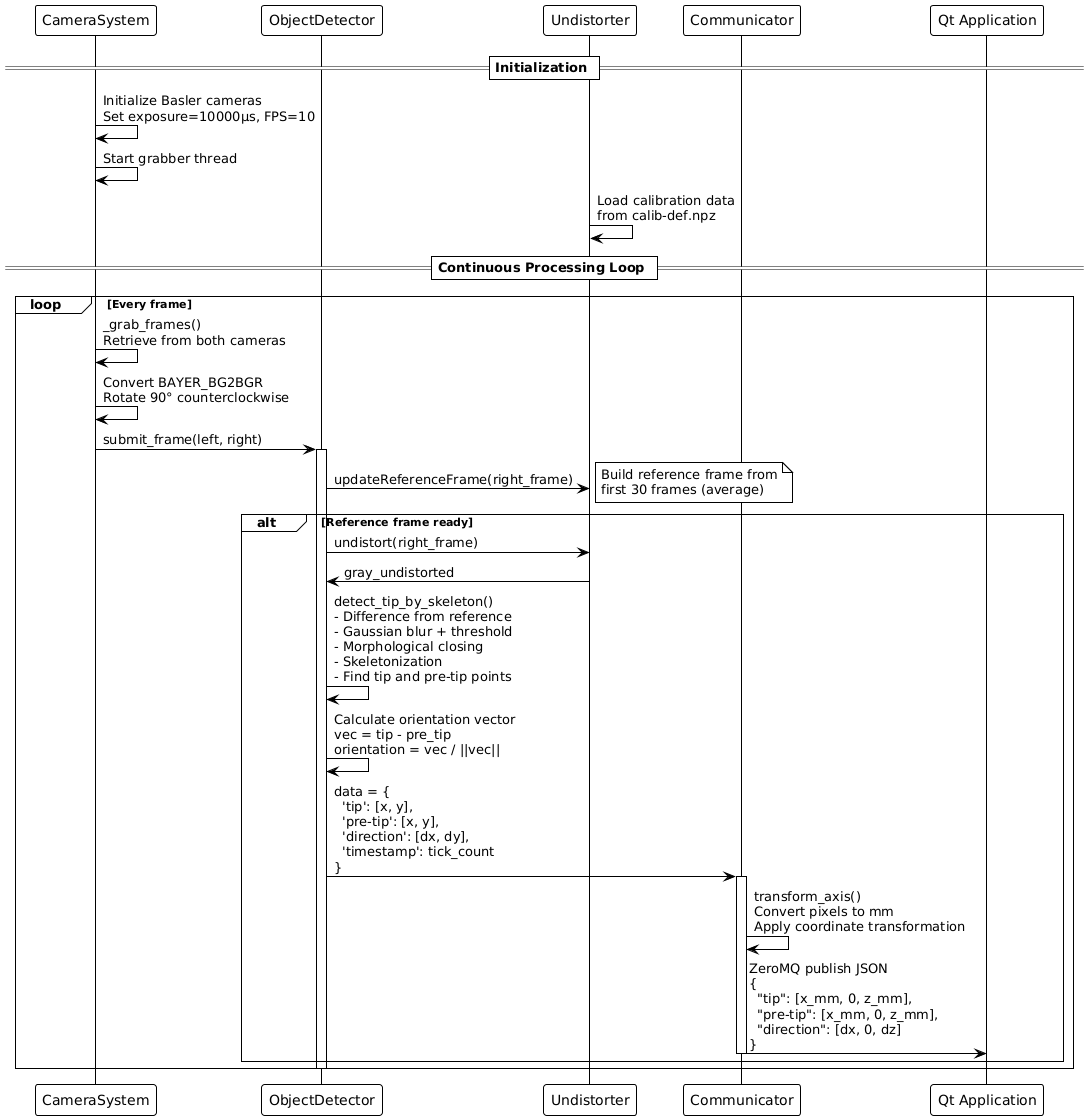
\includegraphics[width=1.1\linewidth]{images/vision/pythonSequencediag.png}
    \caption{Sequence diagram of Python Tip detection code}
    \label{fig:seqpython}
\end{figure}

\todo{figure of vision system detections}

\subsection{Communication Implementation between Python and Qt}


ZeroMQ supports multiple serialization formats, and JSON was chosen for its simplicity and ease of debugging. Each transmitted message consists of a timestamp, the 3D coordinates of the detected tip and pre-tip, and the direction vector. Before transmission, the coordinates undergo a transformation from the coordinate frame utilized in the vision system to the control system's coordinate system. 

The communication system between the vision system (the python tip tracking algorithm) and the controller follows a publisher-subscriber (pub/sub) model. The vision system, acting as the publisher, continuously streams the tip, pre-tip positions and the directional vector data to the ZeroMQ socket bound to the address specified in the \texttt{config} file. There any subscriber on the network can receive updates. 

In the C++/Qt control system a dedicated thread is implemented as a zeroMQ subsciber and listens for vision dta updates. This prevents blocking the main control loop. Once a new message is received the extrancted tip and pre-tip coordinates and direction vector are used as feedback in the control system. This architecture ensures that the control system is always working with the most recent available data while minimizing delays.

\begin{figure} [H]
    \centering
    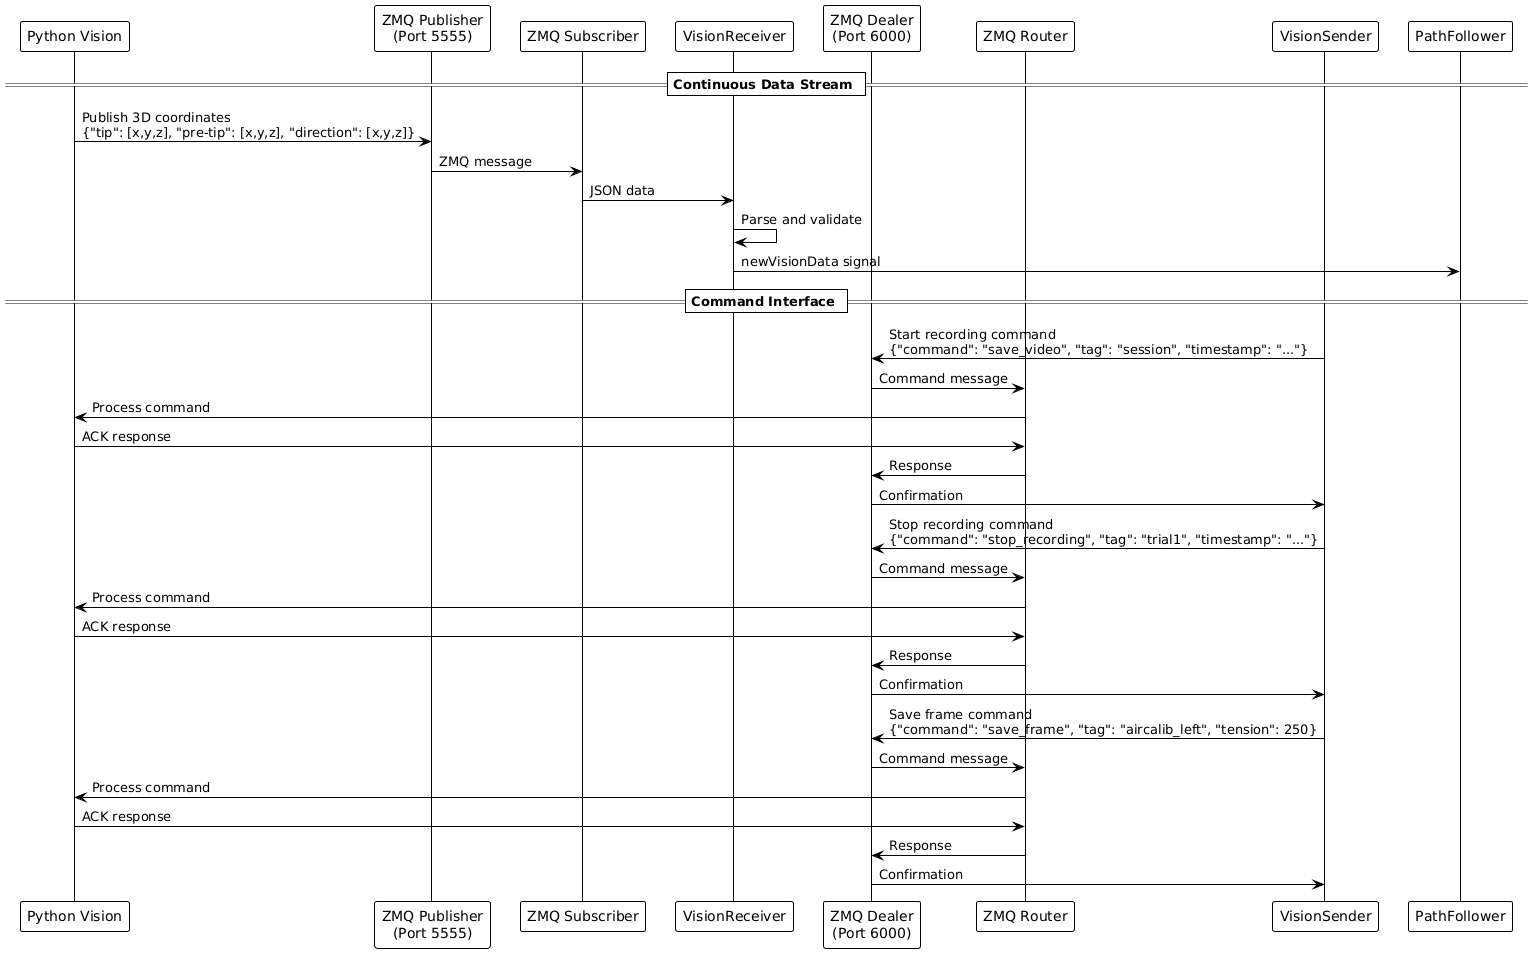
\includegraphics[width=1.1\linewidth]{images/Software documentation/visionSequencediag.png}
    \caption{Sequence diagram of the communication between python vision system and Qt control system}
    \label{fig:seqComm}
\end{figure}

\subsection{Results}
\todo{speed quantification?}

\subsection{Discussion}
This implementation is scalable in the sense that if you want to implement on-line path calculation based on the vision data it can simply also just subscribe to the vision data.

The fact that any subscriber on vision network can receive updates. This ensures flexivbility and allows additional components such as logging or monitoring tools or real time path planning to be added as subscribers in the future.

By leveraging low-latency, connectionless messaging, the system ensures that the most recent vision data is always available without the delays associated with TCP retransmissions or message queues. The pub/sub model further enhances scalability, allowing additional subscribers to be integrated as needed.

By structuring the vision and control system communication in this manner, the system achieves fast, robust, and scalable data exchange while maintaining the flexibility to accommodate future improvements. The combination of efficient data serialization, independent processing threads, and network optimizations ensures that the communication layer operates at a high frequency without compromising the responsiveness of the control system. 


\todo{rewrite whole subsubsection}
